\section{Energy integration}


Nasibeh use cetow for heat puming solutions and st fons for large scale integration and combined heat and power production. We have to use neutralised values (i.e. we start with 100 unit and end up with 46.


Converting energy resources into useful energy, exergy efficiency, heat pumping and combined heat and power => examples from the papers of Nasibeh

adding a citation \cite{Pouransari_2014_1}

testing equations
\begin{equation}
min \, obj= \frac{things_{good}}{things_{bad}} \forall things\\
\text{subject to}  \\
things_{bad}\ge necessary\,\, level \cup unnecessary \, level
\end{equation}

**************

\subsection{Caste study I: Energy integration technologies}

The process heat transfer requirement for a real chemical site is defined using multi-level data extraction approach of \cite{Pouransari_2014_2}. The multi-level data extraction schema includes five levels of growing complexity: \textit{black-box, grey-box, white-box, simple-model} and \textit{detailed-model analysis}. Each level includes the heat transfer requirement with different exergy content. The idea of this approach is to define the energy requirement from different data collection sources including energy conversion, distribution or process units in order to overcome the difficulties of data gathering in large scale plants. Based on the heating and cooling requirement definition performed on the previous section, the Composite and the Grand Composite Curves can be generated such as in \cref{fig1:mer}.

        \begin{figure}[h]
        \begin{center}
        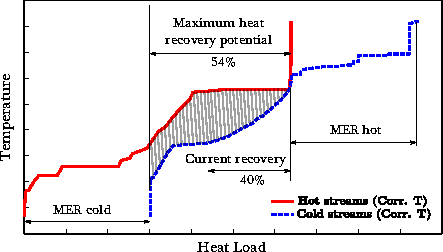
\includegraphics [height=4.3cm]{figures/EnergyIntegration/figMERcc.pdf} 
        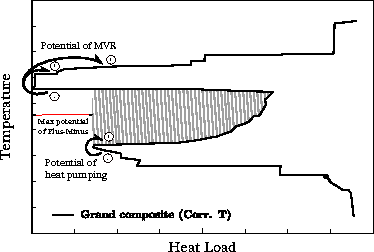
\includegraphics [height=4.3cm]{figures/EnergyIntegration/figMERgcc.pdf}
        \caption{Composite and Grand Composite Curves of the process after heat integration}
        \label{fig1:mer}
        \end{center}
        \end{figure}
        


      \begin{figure}[h]
      \begin{center}
      \begin{tabular}{cc}
        \subfloat[With MVR]{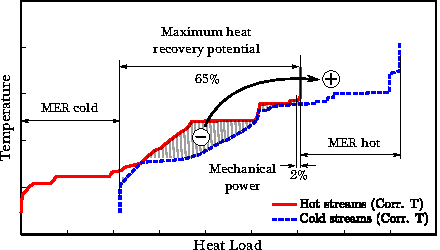
\includegraphics [height=4cm]{figures/EnergyIntegration/HPmvr_mvralone.pdf}} & 
        \subfloat[With MVR and HP]{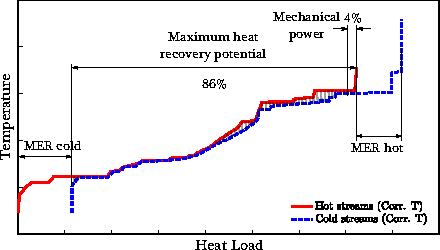
\includegraphics [height=4cm]{figures/EnergyIntegration/HPmvr_mvrhp.pdf}}
       \end{tabular}
      \caption{Composite Curves after improvement potentials}
      \label{fig1:HPmvr}
      \end{center}
      \end{figure}
